\section{\secbitstrings}
\label{sec_bit_strings}

Strings consisting only of \bs{0}s and \bs{1}s, or \vocab{bit strings}, play a central role in computer science. All numbers, data, logical commands, and computer programs are encoded in a computer as bit strings. Similarly, every text message or email message is encoded as a bit string. In fact, we might say that 
\begin{quote}
    Bit strings are a fundamental structure of computer science because all of computer science can be defined using bit strings.   
\end{quote}

In this section, we count bit strings, demonstrate clever ways to count by modeling using bit strings, and discuss exponential notation and logarithms.

%%%%%%%%%%%%%%%%%%%%%%%%%%%%%%%%
\newcommand{\subbitstrings}{Bit Strings}
\subsection{\subbitstrings}
\label{sub_bitstrings}

We start with a definition.

\begin{defn} [Bit string]
\label{defn_bit_string}
~
    \begin{apart}
        \item A character that is \bs{0} or \bs{1} is a \vocab{bit}.
        \item A \vocab{bit string} is a string where each character is a bit. For example, \bs{1101} is a bit string.  
        \item The \vocab{weight} of a bit string is the number of \bs{1}s in the bit string. For example, the bit string \bs{1101} has length four and weight three.
        \item The \vocab{empty bit string} $\lambda$, pronounced ``lambda'', is the unique bit string of length zero.  The symbol $\lambda$ is a place holder.  If we had just a blank space, you would not know that we meant the empty bit string.  In computer science, the empty bit string is used as a start to build a new bit string.  If we start with $\lambda$ and write \bs{1} at the end of the string, the resulting bit string is \bs{1} (and we no longer write $\lambda$).
    \end{apart}  
\end{defn}

Here is an example of listing bit strings using a possibility tree.  

\begin{exam}[Listing bit strings in a possibility tree]
\label{exam_bit_string_length3}
~
    \begin{apart}
        \item List all bit strings of length three by drawing a possibility tree.  
            \begin{soln}
              We draw the possibility tree in \Cref{fig_tree_bit_strings_length3}.  The list is \bs{000}, \bs{001}, \bs{010}, \bs{011}, \bs{100}, \bs{101},\bs{110}, \bs{111}.
        \end{soln}
        
        \begin{figure}[hbtp]
        \centering
        %Used in \Cref{sec_bit_strings}

\begin{tikzpicture}[
    grow=right,
    level distance=2.2cm,
    sibling distance=5.0cm,
    every node/.style={anchor=west},
    level 2/.style={sibling distance=2.5cm},
    level 3/.style={sibling distance=1.3cm}
]
\node {$\bullet$}
    child { node {\texttt{1}}
        child { node {\texttt{1}}
            child { node {$\texttt{0}\to\texttt{110}$} }
            child { node {$\texttt{1}\to\texttt{111}$} }
        }
        child { node {\texttt{0}}
            child { node {$\texttt{1}\to\texttt{101}$} }
            child { node {$\texttt{0}\to\texttt{100}$} }
        }
    }
    child { node {\texttt{0}}
        child { node {\texttt{1}}
            child { node {$\texttt{1}\to\texttt{011}$} }
            child { node {$\texttt{0}\to\texttt{010}$} }
        }
        child { node {\texttt{0}}
            child { node {$\texttt{1}\to\texttt{001}$} }
            child { node {$\texttt{0}\to\texttt{000}$} }
        }
    };
\end{tikzpicture}
        \caption{The possibility tree of all bit strings of length three.}
        \label{fig_tree_bit_strings_length3}
        \end{figure}

        \item List all bit strings of length four and weight two. 
            \begin{soln} 
                We draw the possibility tree in \Cref{fig_tree_bit_strings_length4_weight2}. Each bit string has weight two, which means that it has exactly two \bs{1}s and two \bs{0}s.  In the tree we need to be careful-- any time we have two \bs{1}s or two \bs{0}s, we have only one branch (either to just \bs{0} or to just \bs{1})  instead of the usual two branches (to \bs{0} and to \bs{1}).  The strings are \bs{0011}, \bs{0101}, \bs{0110}, \bs{1001}, \bs{1010}, \bs{1100}.
    \end{soln}
    
        \begin{figure}[hbtp]
        \centering
        \caption{The possibility tree of all bit strings of length four and weight two.}
        \label{fig_tree_bit_strings_length4_weight2}
        \end{figure}       
    \end{apart}   
\end{exam}

Now it is your turn to work with bit strings.

\begin{act} [Listing bit strings]
\label{act_listing_bit_strings}
    ~ 
     \begin{actpart}         
         \item Give an example of a bit string of length four.
         \item Give an example of a bit string of length five and weight three.
         \item \label{part_tree_bs4} List all bit strings of length four using a possibility tree.  Be sure to include the list itself.
         \item Make a table showing the number of bit strings of length $n$ for $n= 1, 2, 3, 4$.  Hint: You can count the answers in your possibility tree from (\ref{part_tree_bs4}).   
         \item Based on the values in your table, how many bit strings of length five should there be?
         \item Explain how you can use steps (\Cref{thm_steps_multiply}) to count the number of bit strings of length five. Did you get the same answer?
         \item Conjecture the number of bit strings of length $n$.        
         \item \label{part_bit_strings_length5_weight3} List the bit strings of length five and weight three by drawing a possibility tree. Your tree should include only those bit strings.
    \end{actpart}
\end{act}

%%%%%%%%%%%%%%%%%%%%%%%%%%%

\newcommand{\subcountbitstrings}{Number of Bit Strings}
\subsection{\subcountbitstrings}
\label{sub_count_bit_strings}

One special situation that is counted using steps is the number of bit strings of length $n$.  Make sure that you have completed \Cref{act_listing_bit_strings} because we are about to reveal the answers.

\begin{exam} [Conjecture number of bit strings of length $n$]
\label{exam_conjecture_number_bit_strings}
    How many bit strings of length $n$ are there?  State your answer as a conjecture.
    \begin{soln}
        There is one bit string of length 0 ($\lambda$), two bit strings of length one (\bs{0}, \bs{1}) and four bit strings of length two (\bs{00}, \bs{01}, \bs{10}, \bs{11}).  In \Cref{exam_bit_string_length3}, we listed the eight bit strings of length three.  In \Cref{act_countingbs}, we counted 16 bit strings of length four and 32 bit strings of length five. Notice that each integer is twice the previous number, suggesting that we are multiplying by two.  \Cref{table_number_bit_strings} shows these examples written as a product of twos.
        
        \begin{table}[htbp]   
            \centering
            \begin{tabular}{l|l}
                $n$ & Number of bit strings of length $n$. \\ \hline
                0 & 1 \\ \hline
                1 & $2 = 2$ \\ \hline
                2 & 4 = $2 \times 2$ \\ \hline
                3 & $8 = 2 \times 2 \times 2$ \\ \hline
                4 & $16 = 2 \times 2 \times 2 \times 2$ \\ \hline
                5 & $32 = 2 \times 2 \times 2 \times 2 \times 2$ \\ 
            \end{tabular}
        \caption{The number of bit strings of length $n$ for $n=1,2,3,4,5$.}       
        \label{table_number_bit_strings}
        \end{table}
        Based on these examples, it is reasonable to conjecture that there are 
        $$\underbrace{2 \times 2 \times \ldots \times 2}_{n \text{ times}}$$
        bit strings of length $n$. 
    \end{soln}   
\end{exam}

Products in the format of the answer to \Cref{exam_conjecture_number_bit_strings} occur often enough that they have a name and notation.  
For example, our product is 2 \vocab{to the power of} $n$ which is denoted 
    $$2^n=
    \underbrace{2\times 2 \times \ldots \times 2}
    _{n \text{ times}}.$$
 
We can prove our conjecture from \Cref{exam_conjecture_number_bit_strings} using steps. 

\begin{thm} [Number of bit strings of length $n$]
\label{thm_number_bit_strings} 
~
    There are $2^n$ bit strings of length $n$.
    \begin{proof}
        Imagine building each bit string of length $n$ by filling in the $n$ spaces:
            $$\underline{\quad}~\underline{\quad}
        ~\underline{\quad}~\ldots
        ~\underline{\quad}~$$
        There are two ways to fill in each space: either \bs{0} or \bs{1}. We fill in the spaces in a sequence of steps. 
        
        Step 1: Fill in the first space (2 ways).  
        
        Step 2: Fill in the second space (2 ways).  
        
        Step 3: Fill in the third space (2 ways). 
        
        We continue to fill spaces until Step $n$: Fill in the last space (2 ways).  
        
        Since steps multiply (\Cref{thm_steps_multiply}), the total number of bit strings of length $n$ is 
        $$\underbrace{
        2 \times 2 \times \ldots \times 2}
        _{n \text{ times}}
        = 2^n.$$
    \end{proof}
\end{thm}

Let's practice counting bit strings.

\begin{act} [Counting bit strings]
\label{act_countingbs}  
~
    \begin{actpart}
        \item How many bit strings of length eight are there?
        \item How many bit strings of length eight and weight one are there?  Hint: How many places are there for the one \bs{1}?
        \item \label{part_bs_length8_weight2} How many bit strings of length eight and weight two are there?  Hint: We can build such a bit string by putting a \bs{0} or \bs{1} in each of eight spaces:
          $$\underline{\quad}~\underline{\quad}~\underline{\quad}~\underline{\quad}~\underline{\quad}~\underline{\quad}~\underline{\quad}~\underline{\quad}~$$

        but we need exactly two spaces to have \bs{1} so filling in the spaces from left to right will not work and there are too many to draw a possibility tree.  Instead, consider choosing which two spaces to fill in with \bs{1}.  Since the remaining spaces are \bs{0}s, the number of bit strings of length eight and weight two equals the number of ways to choose the two spaces for \bs{1}s.
        \item Conjecture the number of bit strings of length $n$ with weight $k$ or, equivalently, exactly $k$ \str{1}s.          
    \end{actpart}
\end{act}

Sometimes, a counting problem asks about subsets of a set, which is convenient because $\binom{n}{k}$ counts the number of $k$-element subsets of a set of $n$ elements. As we saw in \Cref{act_countingbs}, a counting problem might have nothing to do with subsets, but we can rephrase the problem in terms of subsets.  Here is another example.

\begin{exam} [Bit strings of length 100 and weight three]
\label{exam_bit_strings_length100_weight3}
    How many bit strings of length 100 and weight three are there?  

    \begin{soln}
        Let's figure out a way to rephrase this problem in terms of subsets.  We can build such a bit string by putting a \bs{0} or \bs{1} in each of 100 spaces:
        $$\underline{\quad}~\underline{\quad}~\underline{\quad}~\underline{\quad}~\underline{\quad}~\underline{\quad}~\underline{\quad}~\underline{\quad}~\underline{\quad}~\underline{\quad}~\underline{\quad}~\underline{\quad}~\underline{\quad}~\underline{\quad}~\underline{\quad}~\ldots~\underline{\quad}~\underline{\quad}.$$

        Following the hint in \Cref{act_countingbs}, let's choose which spaces have \bs{1}s.
        
        Step 1: Fill in three spaces with \bs{1}.  We choose a subset of three spaces for \bs{1}s from the set of 100 spaces. There are $\binom{100}{3}$ ways to do this step.

        Step 2: Fill in the remaining 97 spaces with \bs{0}.  There is one way to do this step because the 97 \str{0}s go into the remaining 97 spaces.  Alternatively, you can think of choosing a subset of 97 spaces for the \bs{0}s from the set of 97 remaining spaces.  There are $\binom{97}{97} =1$ ways to do this step.

        Since steps multiply (\Cref{thm_steps_multiply}), there are $\binom{100}{3}(1) = \binom{100}{3}$ bit strings of length 100 and weight three.  Our final answer is $\binom{100}{3}$, which a quick internet search shows equals \text{161,700}, too many to list by hand!
    \end{soln}    
\end{exam}

We can generalize our answer and rationale from \Cref{exam_bit_strings_length100_weight3}, to get a formula for the number of bit strings of length $n$ with exactly $k$ \str{1}s (or with exactly $k$ \str{0}s).

\begin{thm}[Number of bit strings of length $n$ with exactly $k$ \str{1}s (or with exactly $k$ \str{0}s).]
\label{thm_bit_string_exactly_k}
The number of bit strings of length $n$ with exactly $k$ \str{1}s (or with exactly $k$ \str{0}s) is $\binom{n}{k}$. 
\end{thm}

Let's see this theorem in action.

\begin{exam}[Counting bit strings with given number of \bs{0}s or \bs{1}s]
\label{exam_count_bs_exactlyk}
~
    \begin{apart}
        \item Count the number of bit strings of length five and weight three.  
            \begin{soln}
                By \Cref{thm_bit_string_exactly_k}, there are $\binom{5}{3}$ bit strings of length five and weight three.  Note that $\binom{5}{3}=10$, which should agree with the tree you drew in \Cref{act_listing_bit_strings} (\ref{part_bit_strings_length5_weight3}).
            \end{soln}
        \item Count the number of bit strings of length eight and weight two. 
            \begin{soln}
                By \Cref{thm_bit_string_exactly_k}, there are $\binom{8}{2}$ bit strings of length eight and weight two, which is the answer to \Cref{act_countingbs}(\ref{part_bs_length8_weight2}). 
            \end{soln}
        \item How many bit strings of length 100 are exactly half \bs{0}s and half \bs{1}s?
            \begin{soln}
                By \Cref{thm_bit_string_exactly_k} there are $\binom{100}{50}$ such bit strings.
            \end{soln}
    \end{apart}        
\end{exam}

%%%%%%%%%%%%%%%%%%%%%%%%%%%%%%%%%%%%%%%%

\newcommand{\subrephrasingsubset}{Detour: Rephrasing the Question}
\subsection{\subrephrasingsubset}
\label{sub_rephrasing_subset}

Sometimes a counting problem does not mention bit strings, but we can rephrase the problem in terms of bit strings, which is convenient because we know \Cref{thm_number_bit_strings} and \Cref{thm_bit_string_exactly_k}.  Try your hand at such an example.

\begin{act} [From point $a_1$ to point $c_4$]
\label{act_froma1_toc4}  
    In this activity we are interested in direct paths from $a_1$ to $c_4$ in \Cref{fig_froma1_toc4}. We begin each direct path at $a_1$ and then walk one unit to the right or one unit down at each step until we reach $c_4$. We are not allowed to walk to the left or up.

    \begin{figure}[hbtp]
        \centering
            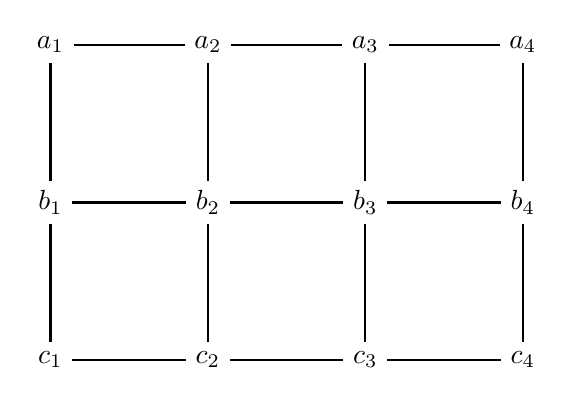
\begin{tikzpicture}[
    colorstyle/.style={
       circle, draw=white,fill=none,
       thick, inner sep=2pt, minimum size=1 mm,
       outer sep=0pt
        },
    scale=2]

\foreach [count=\j] \x in {0,...,3} {
   \node (n-1-\j) at (\x,0) {$c_\j$};
   \node (n-2-\j) at (\x,1) {$b_\j$};
   \node (n-3-\j) at (\x,2) {$a_\j$};
   \draw [thick] (n-1-\j) -- (n-2-\j);
   \draw [thick] (n-2-\j) -- (n-3-\j);
  }
\foreach [remember=\i as \j (initially 1)] \i in {2,...,4} {
   \draw [thick] (n-1-\j) -- (n-1-\i);
   \draw [thick] (n-2-\j) -- (n-2-\i);
   \draw [thick] (n-3-\j) -- (n-3-\i);
 }
\end{tikzpicture}
        \caption{Going from point $a_1$ to point $c_4$.}
        \label{fig_froma1_toc4}
    \end{figure}

    \begin{actpart}
        \item Give an example of a direct path from $a_1$ to $c_4$.  How many steps did you take?
        \item \label{part_froma1_toc4_tree} Draw a possibility tree to list all possible direct paths. Hint: The original node is $a_1$ which has branches to $a_2$ and to $b_1$.   
        \item \label{part_froma1_toc4_count} How many direct paths from $a_1$ to $c_4$ are there?
        \item We can represent each path by a bit string where \bs{1} represents walking one unit to the right and \bs{0} represents walking one unit down.  What is the bit string whose path is $a_1a_2b_2b_3c_3c_4$?
        \item What is the path whose bit string is $\bs{00111}$?
        \item Explain how to use \Cref{thm_bit_string_exactly_k} to count the number of paths. You should get the same answer as in (\ref{part_froma1_toc4_count}).
        \item We can describe the grid in \Cref{fig_froma1_toc4} as being $3 \times 4$ because it has 3 rows of letters and 4 columns of letters.  Conjecture the number of direct paths from the upper left corner to the lower right corner in a $5 \times 7$ grid.
        \item Generalize. That means conjecturing the number of direct paths from the upper left corner to the lower right corner in a $r \times c$ grid.
    \end{actpart}
\end{act}

%%%%%%%%%%%%%%%%%%%%%%%%%%%%%%%%%%%%%%%%%%%%%

\newcommand{\subexplog}{Algebra: Exponential Notation and Logarithms}
\subsection{\subexplog}
\label{sub_exp_log}

In \Cref{thm_number_bit_strings}, we proved that there are $2^n$ bit strings of length $n$ where
$$2^n=\underbrace{2\times 2 \times \ldots \times 2}_{n \text{ times}}$$
This \vocab{exponential notation} is a shorthand for a product of the same number multiplied by itself repeatedly.

\begin{defn} [Exponential notation]
\label{defn_exp_notation}
~
    \begin{apart}
        \item When $n$ is a positive integer, $b$ \vocab{raised to the power of} $n$ (or just $b$ \vocab{to the} $n$) is
        $$b^n = \underbrace{b\times b \times \ldots \times b}_{n \text{ times}}$$
        For example, 
        $$2^5 = \underbrace{2 \times 2 \times 2 \times 2 \times 2}_{5 \text{ times}} = 32$$ 
        and 
        $$(-2)^5 = \underbrace{(-2) \times (-2) \times (-2) \times (-2) \times (-2)}_{5 \text{ times}} = -32.$$ 
        Note that exponentiation is not commutative.  For example, $2^5=32$ but $5^2 = 5 \times 5 = 25$.  We practice evaluating powers without using technology to understand the definition, but, of course, you can use technology to check.  Many computational tools, such as calculators, spreadsheet programs, or an Internet search, use the notation $\land$ to indicate a power.
        \item In the expression $b^n$, the integer $b$ is the \vocab{base}, the number that we are repeatedly multiplying.  The integer $n$ is the \vocab{exponent}, the number of times we multiply the base.  The quantity $b^n$ is the \vocab{power of} $b$, the final product.  For example, in $2^5$, the base is 2, the exponent is 5, and the power of 2 is 32.  
        \item For $b\neq 0$, it is convenient to define $b^0=1.$  For example, $2^0=1$ is the number of bit strings of length zero.
        \item The expression $b^2$ is $s$ \vocab{squared}.  For example, $10^2 = 10 \times 10 = 100$. This name comes from the fact that the area of a square with sides of length $b$ is $b^2$.
        \item The expression $b^3$ is $b$ \vocab{cubed}.  For example, $4^3 = 4 \times 4 \times 4 = 64$. This name comes from the fact that the volume of a cube with sides of length $b$ is $b^3$.  
     \end{apart}
\end{defn}

Let's work with these definitions.

\begin{exam} [Exponential notation]
\label{exam_exponential notation}
    In this example, we only use technology to check our answers.
    \begin{apart}
        \item Evaluate $10^4$. 
            \begin{soln}
                By definition, 
                \begin{center}
                    \begin{tabular}{lll}
                       $10^4$ &=& $\underbrace{10 \times 10 \times 10 \times 10}_{4 \text{ times}}$ \\
                       &=& $100 \times 10 \times 10 $ \\
                       &=& 1,000 $\times 10$ \\
                       &=& 10,000. \\    
                   \end{tabular}
                \end{center}
               Check that $10 \land 4 =$ 10,000.  Notice that $10^4$ has 4 zeros.
            \end{soln}  
        \item Evaluate $(-10)^4$ and $-10^4$.
            \begin{soln}
                By definition, 
                \begin{center}
                    \begin{tabular}{lll}
                       $(-10)^4$ &=& $\underbrace{(-10) \times (-10) \times (-10) \times (-10)}_{4 \text{ times}}$ \\
                       &=& $100 \times (-10) \times (-10) $ \\
                       &=& -1,000 $\times (-10)$ \\
                       &=& 10,000. \\    
                   \end{tabular}
                \end{center}
                Check that $(-10) \land 4 = \text{10,000}$.
                On the other hand, according to \Cref{defn_integer_algebra_order_operations} (\ref{part_order_operations}), exponents are higher in the order of operations in  than subtraction (and negation), so 
                    $$-10^4=-(10^4)=-\text{10,000}.$$
                Check that $-10 \land 4 = -\text{10,000}$.
            \end{soln}
        \item Evaluate $3^1$. 
             \begin{soln}               
                 By definition, $$3^1 = \underbrace{3}_{1 \text{ time}} = 3.$$
                Check that $3 \land 1 = 3.$
            \end{soln}
        \item Evaluate $5^0$.
            \begin{soln}
                By definition, $5^0 =1$ and check that $5 \land 0 =1$. 
            \end{soln}

    \end{apart}    
\end{exam}

It can be useful to write an integer as a power of a base $b$.  For example, we can write $\text{10,000}=10^4$ or $32 = 2^5$.  There is a name for the exponent.  

\begin{defn}[Logarithm\footnote{In this textbook, we only calculate logarithms of exact powers.  We do not calculate quantities such as $\fn{log}(25)$ or $\fn{lg}(3)$.  We have defined $b^n$ when $n$ is a nonnegative integer, but it is beyond the scope of this textbook to define what $b^x$ for any real number $x$.  With that definition, we can take evaluate logarithms of any positive real number.  For example, $\fn{log}(25) \approx 1.398$ and $\fn{lg}(3) \approx 1.585$.}]
\label{defn_log}
~
    \begin{apart}
        \item The \vocab{logarithm base 10} of an integer $k$, denoted $\fn{log}(k)$ is the exponent of the power 10 that equals $k$. That is, $\fn{log}(k)=n$ if $10^n=k$.  For example, $\fn{log}(\text{100}) = 2$ because $10^2=100$.
        \item The \vocab{logarithm base 2} of an integer $k$, denoted $\fn{lg}(k)$, is the exponent of the power of 2 that equals $k$. That is, $\fn{lg}(k)=n$ if $2^n=k$.  For example, $\fn{lg}(32) = 5 $ because $2^5=32$.
        \item In this textbook, we only use base 2 and base 10, but logarithms can be defined in general. The \vocab{logarithm base $b$} of an integer $k$, denoted $\fn{log}_b(k)$ is the exponent of the power of $b$ that equals $k$. That is, $\fn{log}_b(k)=n$ if $b^n=k$.  For example, $\fn{log}_5(125) = 3$ because $5^3=125$.  In this notation, $\fn{log}$ is short for $\fn{log}_{10}$ and $\fn{lg}$ is short for $\fn{log}_2$.  In calculus, a noninteger base $b=e \approx 2.718$ is important. The corresponding logarithm is named \fn{ln}. 
    \end{apart}
\end{defn}

Here are a few more examples.

\begin{exam}[Evaluating logs]
\label{exam_eval_logs}
    In this example, we evaluate without using technology.
        \begin{apart}
          \item Evaluate $\fn{log}(\text{1,000,000})$. 
              \begin{soln}
                  Since $\text{1,000,000}= 10^6$, it follows that $\fn{log}(\text{1,000,000})=6$.
              \end{soln}
          \item Evaluate $\fn{lg}(4)$ and $\fn{lg}(256)$.
              \begin{soln}
                  First, since $2^2=4$, it follows that $\fn{lg}(4)=2$. Next, since $2^8=256$, it follows that $\fn{lg}(256)=8$.
              \end{soln}
        \end{apart}
\end{exam}

Practice working with exponents and logarithms.

\begin{act} [Exponents and logarithms] 
    \label{act_exp_logs}  
    On this problem, only use technology to check your answers.
    \begin{actpart}
        \item Evaluate $10^6$, $3^2$, $10^0$, $2^3$. 
        \item Evaluate $(-3)^2$, $-3^2$, $(-2)^3$, $-2^3$. 
        \item Evaluate $\fn{log}(\text{1,000})$, $\fn{log}(10)$, and $\fn{log}(1)$.
        \item Evaluate $\fn{lg}(16)$, $\fn{lg}(\text{128})$, and $\fn{lg}(2)$.
        %%%
        \item Find an integer $k$ such that $\fn{log}(k) = 10$.       
        \item Find an integer of $n$ such that $\fn{lg}(n) = 10$.
        \item Simplify $2^32^5$ by writing it as a single power.
        \item Simplify $(2^3)^2$ by writing it as a single power.
        \item Simplify $2(2^{n-1})$ by writing it as a single power. 
     \end{actpart}
\end{act}

Let's look at examples of writing a combination of powers as a single power.

\begin{exam}[Simplifying exponents]
\label{exam_simplify_exponents}
~
     \begin{apart}
         \item Simplify $2^42^6$ by writing it as a single power.
             \begin{soln}
                 Using \Cref{defn_exp_notation}, we have
                     \begin{align*}
                         2^42^6 &= (\underbrace{2\times 2\times 2 \times 2}_{4 \text{ times}}) \times
                         (\underbrace{2\times 2\times 2 \times 2 \times 2 \times 2}_{6 \text{ times}}) \\
                         &= \underbrace{2\times 2\times 2\times 2\times 2 \times 2 \times 2 \times 2 \times 2 \times 2}_{10 \text{ times}}) \\ 
                         &= 2^{10}.
                    \end{align*}
                Notice that the base remains 2 and that since the powers shared a common base, the exponents added: $4+6=10$.
             \end{soln}
        \item \label{part_power_of_power} Simplify $(10^2)^3$ by writing it as a single power.
            \begin{soln}
                Using \Cref{defn_exp_notation}, we have
                     \begin{align*}
                         (10^2)^3 &= (\underbrace{10^2\times 10^2\times 10^2}_{3 \text{ times}}) \\
                         &= (\underbrace{(10 \times 10)\times (10 \times 10)\times (10 \times 10)}_{3 \text{ times}}) \\
                         &= \underbrace{10\times 10\times 10\times 10\times 10 \times 10}_{6 \text{ times}}) \\ 
                         &= 10^6.
                    \end{align*}
                Notice that the exponents multiplied: $2 \times 3=6$.
            \end{soln}
        \item Write $8^2$ as a power of 2.
            \begin{soln}
                First, write $8 = 2^3$.  Then, using what we learned in (\ref{part_power_of_power}) we get
                    $$8^2=\left(2^3\right)^2 = 2^{2\times 3}=2^6.$$
                You can check that $8^2=64$ and $2^6=64$.
            \end{soln}
     \end{apart}
\end{exam}

We state these rules for exponents as a theorem, but, when in doubt, we suggest that you use the definition instead.

\begin{thm}[Simplifying exponents]
\label{thm_simplify_exp}
    For any integer $b$ and positive integers $n$ and $m$ we have the following rules.
        \begin{apart}
            \item Simplifying a product of powers (of the same base): $b^mb^n=b^{m+n}$.
            \item Simplifying a power of a power: $\left(b^m\right)^n=b^{mn}$.
        \end{apart}
\end{thm}

Here is an example of a common expression that we can simplify using these rules.

\begin{exam}[Simplify $2\cdot2^{n-1}$]
\label{exam_simplify_22nminus1}   
~
    \begin{apart}
        \item \label{part_thm_simplify_22nminus1} Simplify $2\cdot2^{n-1}$ using \Cref{thm_simplify_exp}.
            \begin{soln}
                We can write $2=2^1$ to get
                    $$2\cdot2^{n-1} = 2^12^{n-1}=2^{1+(n-1)}=2^n.$$
            \end{soln}
        \item Confirm your answer to (\ref{part_thm_simplify_22nminus1}) using the definition of exponents.
            \begin{soln}
                We can write 
                    $$2\cdot2^{n-1} 
                    = 2 \times 
                    \underbrace{2 \times 2 \times \cdots \times 2}_{(n-1) \text{ times}} 
                    = \underbrace{2 \times 2 \times \cdots \times 2}_{n \text{ times}}
                    =2^n$$
            \end{soln}
    \end{apart}
\end{exam}

It is acceptable to leave exponential notation or logarithms in your answers.

\begin{rem} [Not evaluating counts, final version]
\label{rem_not_eval_counts_final}
Unless stated otherwise, when counting you may leave any answer greater than twenty in a format that could easily be evaluated on a calculator. In particular, your answer may involve addition, subtraction, multiplication, division, exponents, logarithms, factorials, binomial coefficients, and parentheses.
\end{rem}

%%%%%%%%%%%%%%%%%%%%%%%%%%%%%%%%%%%%%%%%%%%%

\subsection{Exercises}

%%%%%%%%%%%%%%%%%%%%%%%%%%%%%%%%%%%%%%%%%%%%
    
\subsubsection*{Exercises for \Cref{sub_bitstrings} \subbitstrings}

\begin{exer} [\exerP] % length and weight of bit strings]
\label{exer_bit_string_length}
    ~
    \begin{exerpart}
         \item Calculate the length and weight of the bit string \bs{101100}.
        \item Calculate the length and weight of the bit string \bs{0}.
        \item Give an example of a bit string of length ten and weight four.  
    \end{exerpart}
\end{exer}

\begin{exer} [\exerP] % bit strings of length five and weight two]
\label{exer_bit_strings_length5_weight2}
    List all bit strings of length five and weight two using a possibility tree.
\end{exer}

\begin{exer} [\exerU] %  bit string possibility trees]
\label{exer_bstrees}
    In each part, list all bit strings of length five satisfying the stated property using a possibility tree.  In each case, your tree should only include the bit strings that satisfy the stated property.
    \begin{exerpart}
        \item Bit strings with more \bs{0}s than \bs{1}s.
        \item Bit strings that do not contain consecutive \bs{0}s, which means that \str{00} does not appear in the bit string.
        \item Bit strings where any \bs{0} is immediately followed by \bs{1}.       
    \end{exerpart}   
\end{exer}

\begin{exer}[\exerR] % defn bit strings
\label{exer_dyk_defnbs}
    Do you know \ldots
        \begin{exerpart}
            \item What a bit is?
            \item How to calculate the length of a bit string or construct a bit string of a given weight?
            \item How to calculate the weight of a bit string or construct a bit string of a given weight? 
            \item What the symbol for empty bit string is?
        \end{exerpart}
\end{exer}

\begin{exer}[\exerE] % hamming distance
\label{exer_hamming_distance}  
    The \vocab{Hamming distance} between two bit strings is the number of places where their bits differ.  For example, the Hamming distance between \bs{10011} and \bs{11010} is two because they have the same first bits (both \bs{1}), different second bits, the same third bits (both \bs{0}), the same fourth bits (both \bs{1}), and different fifth bits.  Since the bit strings differ in two places (second and fifth), their Hamming distance equals two.  Hamming distance is used in error-correcting codes to ensure the correct transmission of messages such as text messages.
        \begin{apart}
            \item Calculate the Hamming distance between \bs{00011} and \bs{11111}.
            \item List all bit strings that are Hamming distance one from \bs{00011}.
            \item Give an example of a bit string that is Hamming distance two from \bs{00011}.
            \item If $b$ is any bit string of length five, how many bit strings are Hamming distance one from $b$?  Explain.
            \item If $b$ is any bit string of length five, how many bit strings are Hamming distance two from $b$?  Explain.
        \end{apart}
\end{exer}
%%%%%%%%%%%%%%%%%%%%%%%%%%%%%%%%%

\subsubsection*{Exercises for \Cref{sub_count_bit_strings} \subcountbitstrings}

\begin{exer} [\exerP] % bit strings of length 20]
\label{exer_count_bs20}
    Use the relevant theorems.
        \begin{exerpart}
            \item How many bit strings of length twenty are there?
            \item How many bit strings of length twenty contain exactly three \bs{1}s?
            \item How many bit strings of length twenty contain exactly three \bs{0}s?      
        \end{exerpart}
\end{exer}

\begin{exer} [\exerU] % bit strings of length9]
\label{exer_count_bs9}
    Use the relevant theorems.
        \begin{exerpart}
            \item How many bit strings of length nine are there? 
            \item How many bit strings of length nine or ten are there?  Hint: Use cases.
            \item Which number is greater: the number of bit strings of length nine or the number of bit strings of length less than nine?  Calculate the actual numbers using technology.  Note: do not forget the empty bit string. 
    \end{exerpart}
\end{exer}

\begin{exer}[\exerU] % bit strings beginning with 0s
\label{exer_count_bs100}  
~
    \begin{exerpart}
        \item How many bit strings of length 100 begin with \bs{0}? Explain.
        \item How many bit strings of length 100 begin with \bs{00}? Explain.
        \item How many bit strings of length 100 begin with \bs{1} and end in \bs{0}?
        \item How many bit strings of length 100 begin with or end in \bs{0}?  Hint: To avoid double counting of bit strings that begin with \bs{0} and end in \bs{0}, consider Case 1: begins with \bs{0} and Case 2: begins with \bs{1} and ends in \bs{0}.
    \end{exerpart}
\end{exer}

\begin{exer}[\exerR] % number bit strings
\label{exer_dyk_numberbs}
    Do you know \ldots
        \begin{exerpart}
            \item How many bit strings of length $n$ there are? 
            \item How many bit strings of length $n$ have exactly $k$ \bs{1}s (or exactly $k$ \bs{0}s)?
        \end{exerpart}
\end{exer}

\begin{exer}[\exerE] % balanced ternary strings]
\label{exer_bal_ternary_strings}
    A \vocab{balanced ternary string} is a string where each character is \bs{0}, \str{+}, or \str{-}.  For example, \str{+--0+} is a balanced ternary string of length five.
    \begin{exerpart}
        \item Draw a possibility tree listing all balanced ternary strings of length three.
        \item How many balanced ternary strings of length three are there?
        \item Count the number of balanced ternary strings of length ten.
        \item How many balanced ternary strings of length $n$ are there?  State your answer as a conjecture.
    \end{exerpart}   
\end{exer}

\begin{exer} [\exerE] % \str{ABCD} strings]
\label{exer_ABCD_strings}
    Consider strings using only the characters \str{A}, \str{B}, \str{C}, and \str{D}.  Recall that a string is ordered and repeats are allowed.  Also, we do not need to use all the characters.
    \begin{exerpart}
    \item How many such strings consist of exactly two \str{A}s and three \str{B}s?
    \item How many such strings consist of exactly two \str{A}s, three \str{B}s, and four \str{C}s?
    \item How many such strings consist of exactly two \str{A}s, three \str{B}s, four \str{C}s, and five \str{D}s?
    \end{exerpart}
\end{exer}

\begin{exer} [\exerE] % number of permutations]
\label{exer_number_perms} 
~
    \begin{exerpart}
        \item Conjecture the number of permutations of the set $\{\str{1},\str{2},\ldots, \str{n}\}$.
        \item Prove your conjecture in the style of our proof of \Cref{thm_number_bit_strings}.
    \end{exerpart}
\end{exer}

%%%%%%%%%%%%%%%%%%%%%%%%%%%%%%%%%%%%%%

\subsubsection*{Exercises for \Cref{sub_rephrasing_subset} \subrephrasingsubset}

\begin{exer}[\exerP] % from point $a_1$ to point $c_4$ revisited]
\label{exer_froma1toc4}
    We are interested in going from $a_1$ to $c_4$ in \Cref{fig_froma1_toc4}.  As in \Cref{act_froma1_toc4}, we can represent each path by a bit string where \str{1} represents walking one unit to the right and \str{0} represents walking one unit down.  
        \begin{exerpart}
            \item What is the bit string whose path is $a_1b_1b_2b_3c_3c_4$?
            \item What is the path whose bit string is \bs{11010}?           
        \end{exerpart}
\end{exer}

\begin{exer} [\exerU] % fifteen coins]
\label{exer_stars_and_bars}
    You have fifteen (identical) coins. You want to put some coins in your piggy bank, some in your change jar at work, and some in your car. 
    \begin{exerpart}
        \item How many ways are there to distribute your coins to these three locations?  Note that ``some'' could mean zero in this context.

        Hint: Line up the fifteen coins.  Put a dividing line after those you plan to put in the piggy bank, if any, and another line after those you plan to put in your change jar, if any. The remaining coins, if any, will go in your car. 
        
        For example:  six coins in the piggy bank, two coins in the change jar, and seven coins in the car could be represented as:
            $$\circ ~ \circ ~ \circ ~ \circ ~ \circ ~ \circ ~ \mid ~ \circ ~ \circ ~ \mid ~ \circ ~ \circ ~ \circ~  \circ ~ \circ ~ \circ ~ \circ ~$$
        whereas three coins in the piggy bank and the rest in the change jar would be:
            $$\circ ~ \circ ~ \circ ~ \circ ~ \mid ~ \circ ~ \circ ~  \circ ~ \circ ~ \circ ~ \circ ~ \circ~  \circ ~ \circ ~ \circ ~ \circ ~ \mid ~ $$
    
      Explain how to rephrase our question about the coins as a question about bit strings. Then answer the question. 
    
      Hint to the last part of the hint: squint.
    \item Conjecture about the number of ways to distribute $n$ coins to $k$ locations.
    \end{exerpart}
\end{exer}

\begin{exer}[\exerR] % rephrase question
\label{exer_dyk_rephrase_question}
    Do you know \ldots
        \begin{exerpart}
            \item How to rephrase a question in terms of subsets and why that can be useful? 
            \item How to rephrase a question in terms of bit strings, and why that can be useful? 
        \end{exerpart}
\end{exer}

\begin{exer} [\exerE] % integer solutions]
\label{exer_integer_simplex}
    In this problem we build on the ideas of \Cref{exer_stars_and_bars}.
    \begin{exerpart}
         \item How many nonnegative integer solutions are there to the equation $x_1+x_2+x_3=15?$  
         Hint: how can we rephrase this question to be the same as the question in \Cref{exer_stars_and_bars}?
         \item How many non-negative integer solutions are there to the equation $x_1+x_2+x_3+x_4=20?$
         \item Make a conjecture about the number of non-negative integer solutions of the equation 
         $x_1+x_2+x_3+\ldots x_k=n$    
    \end{exerpart}
\end{exer}

%%%%%%%%%%%%%%%%%%%%%%%%%%%%%%%%%%%%%%%%%%%%

\subsubsection*{Exercises for \Cref{sub_exp_log} \subexplog}

\begin{exer} [\exerP] % evaluate powers]
\label{exer_evaluate_powers}
     On this exercise, do not use technology.  Be sure to show some work.
     \begin{exerpart}
         \item Evaluate $2^4$, $(-2)^4$, and $-2^4$.
         \item Evaluate $10^{10}$.
         \item Evaluate $4^1$ and $4^0$.
     \end{exerpart}
\end{exer}


\begin{exer}[\exerP] % evaluating logarithms]
\label{exer_eval_logs} 
    On this exercise, do not use technology.  Be sure to show some work. 
        \begin{exerpart} 
            \item Evaluate $\fn{log}(\text{10,000})$, $\fn{log}(10)$, and $\fn{log}(1)$.
            \item Find a value $n$ such that $\fn{log}(n) = 3$.
            \item Evaluate $\fn{lg}(64)$, $\fn{lg}(16)$, $\fn{lg}(2)$, and $\fn{lg}(1)$.
            \item Find a value of $n$ such that $\fn{lg}(n) = 3$. 
        \end{exerpart}
\end{exer}

\begin{exer} [\exerU] % write as a single power]
\label{exer_single_power}  
    Write each quantity as a single power.
    \begin{exerpart}
        \item $k \times k$
        \item $m^2m^7$
        \item $2 (2^9)$
        \item \label{part_10power} $10(10^{n-1})$
        \item \label{part_another_10power} $10(10^n)$
    \end{exerpart}
\end{exer}

\begin{exer} [\exerU] % factoring powers]
\label{exer_factoring_powers}
In this problem, all letters represent positive integers.
    \begin{exerpart}
        \item Factor $n^3 + 3n^2$
        \item Factor $k2^k -2^k$.
        \item Factor and simplify $10^n-9(10^{n-1})$.  Hint: See \Cref{exer_single_power} (\ref{part_10power}) and (\ref{part_another_10power}).
    \end{exerpart}
\end{exer}

\begin{exer}[\exerR] % exponents and logs
\label{exer_dyk_exp_log}
    Do you know \ldots
        \begin{exerpart}
            \item What $b^n$ means and how to pronounce it?
            \item How to pronounce $n^2$ and $n^3$?
            \item How to evaluate $5^0$, $5^1$, and $5^2$?
            \item Where exponents rank in the order of operations?
           \item What $\fn{log}$ and $\fn{lg}$ mean and how to evaluate them?
           \item How to rewrite a statement involving logs as a statement involving exponents? 
        \end{exerpart}
\end{exer}

\begin{exer}[\exerE] % 2048 game]
\label{2048 game}
~
    \begin{exerpart}
        \item Play the online game \vocab{2048} at \url{https://play2048.co/}.  Report here how long you played and how high a level you achieved. Try to get to at least 128.
        \item List the powers of 2 from 1 to 2048 from memory (that is, not using any technology or computing any products).
    \end{exerpart}
\end{exer}

\begin{exer}[\exerE] % definition of $\fn{lg}$]
\label{exer_defn_lg}  
~
    \begin{exerpart}
        \item Write the exponential equation corresponding to $\fn{lg}(128) = 7$.
        \item \label{part_lg_to_exp} For numbers $u$ and $v$, write $a=\fn{lg}(u)$ and $b=\fn{lg}(v)$. Write the corresponding exponential equations.
        \item \label{part_2tosum} Simplify $2^{a+b}$ using \Cref{thm_simplify_exp} and (\ref{part_lg_to_exp}).  Your answer should be in terms of $u$ and $v$.        
        \item \label{part_lg_product} Use your answer to (\ref{part_2tosum}) to evaluate $\fn{lg}(uv)$.  Your answer should be in terms of $a$ and $b$.
        \item Use your answer to (\ref{part_lg_product}) to write $\fn{lg}(uv)$ in terms of $\fn{lg}(u)$ and $\fn{lg}(v)$. Your answer is one of the rules known as a ``law of logs''.
    \end{exerpart}
\end{exer}

\begin{exer}[\exerE] % power vs. factorial]
\label{exer_power_vs_factorial} 
~
    \begin{exerpart}
        \item Without calculating values, decide which is larger: $10!$ or $2^{10}$.  Hint: Use the definitions of factorials and powers to write each of $10!$ and $2^{10}$ as a product. Then use those products to answer the question.
        \item Calculate $10!$ and $2^{10}$ using technology. Did you correctly determine which integer is larger?
        \item Make a table for $n = 0, 1, 2, \ldots, 10$ showing the values of $2^n$ and the values of $n!$. Challenge yourself to reciting the powers of two and as many factorials as you can from memory, but then you are welcome to use computing technology. Hint: Use three rows labeled $n$, $2^n$, and $n!$.
        \item Conjecture when $n! \ge 2^n$. 
    \end{exerpart}
\end{exer}

%%%%%%%%%%%%%%%%%%%%%%%%%%%
\subsection{\answers}
%%%%%%%%%%%%%%%%%%%%%%%%%%%

\subsubsection{\answers for \Cref{sub_bitstrings} \subbitstrings}

\subsubsection*{\Cref{exer_bit_string_length} \answers}
\begin{apart}
    \item Length six and weight three.
    \item Length one and weight zero.
    \item Hint: your bit string should have four \bs{1}s and six \bs{0}s.
\end{apart}

\subsubsection*{\Cref{exer_bstrees} \answers}
\begin{apart}
    \item Hint: Start the possibility tree with two branches to \bs{0} and \bs{1}, as usual.  Next, branch to \bs{0} and \bs{1} again.  After that, you need to be careful. If you ever have two \bs{1}s then the remainder of the bits are all \bs{0}s.  There are 16 such bit strings. One is all \bs{0}s, five that have four \bs{0}s, and ten that have three \bs{0}s.
    \item Hint: Start the possibility tree with two branches to \bs{0} and \bs{1}, as usual. After that, you need to be careful.  After every \bs{1} there are still two branches (to \bs{0} and to \bs{1}), but after every \bs{0} there is a single branch to \bs{1}.
    \item Hint: This part is similar to (b), except that the bit string must end in \bs{1} because a final \bs{0} would not be immediately followed by \bs{1}.
\end{apart}

\subsubsection*{\Cref{exer_hamming_distance} \answers}
\begin{apart}
    \item Three
    \item \bs{10011}, \bs{01011}, \ldots, \bs{00010} Note that these are organized by which bit is different: first, second, \ldots, fifth
    \item Hint: check that exactly two bits are different.
    \item Hint: See the note under (b).
    \item Hint: We need to choose which two out of five bits to change.  
\end{apart}

%%%%%%%%%%%%%%%%%%%%%%%%%%%
\subsubsection{\answers for \Cref{sub_count_bit_strings} \subcountbitstrings}

\subsubsection*{\Cref{exer_count_bs20} \answers}
\begin{apart}
    \item $2^{20}$
    \item $\binom{20}{3}$
    \item Hint: There are two ways to do this problem.  We can choose the three places out of 20 for the \bs{0}s or we can choose the 17 places out of 20 for the \bs{1}.  Either answer is correct.
\end{apart}

\subsubsection*{\Cref{exer_count_bs100} \answers}
\begin{apart}
    \item $2^{99}$. Hint: Steps multiply (\Cref{thm_steps_multiply}).
    \item Hint: There are $100-2=98$ spaces left to fill in.
    \item Hint: Use the hint from (b).
    \item Hint: Case 1 is similar to (b) and case 2 is exactly (c).  Cases add (\Cref{thm_cases_add}). 
\end{apart}

\subsubsection*{\Cref{exer_ABCD_strings} \answers}
\begin{apart}
    \item Hint: Step 1 is to choose two of the five spaces for the \str{A}s.  Step 2 is to choose three of the three remaining spaces for the \str{B}s.  Note that there is only one way to do Step 2 (so you can safely ignore it).
    \item One way of stating the answer is $\binom{9}{2}\binom{7}{3}\binom{4}{4}$.
    \item Hint: Figure out how we got the answer to (b) and generalize.
\end{apart}

%%%%%%%%%%%%%%%%%%%%%%%%%%%
\subsubsection{\answers for \Cref{sub_rephrasing_subset} \subrephrasingsubset}

\subsubsection*{\Cref{exer_froma1toc4} \answers}
\begin{apart}
    \item \bs{01101}
    \item $a_1a_2a_3b_3\ldots$
\end{apart}

\subsubsection*{\Cref{exer_stars_and_bars} \answers}
\begin{apart}
    \item Hint: Each coin is \bs{0} and each dividing line is \bs{1}.  Note that the total length is $15+2=17$.
    \item Hint: The total length is $n+k-1$ because we only need $k-1$ dividing lines.
\end{apart}

\subsubsection*{\Cref{exer_integer_simplex} \answers}
\begin{apart}
    \item $\binom{17}{2}$
    \item Hint: Let $x_1$ be the number of coins in the first location, $x_2$ be the number of coins in the second location, $x_3$ be the number of coins in the third location, and $x_4$ be the number of coins in the fourth location. Count the total number of coins and the number of dividing lines.
    \item Hint: Count the total number of coins and the number of dividing lines.
\end{apart}

%%%%%%%%%%%%%%%%%%%%%%%%%%%
\subsubsection{\answers for \Cref{sub_exp_log} \subexplog}

\subsubsection*{\Cref{exer_evaluate_powers} \answers}
\begin{apart}
    \item Hint: Use a calculator to check.
    \item \text{10,000,000,000}
    \item Hint: Use a calculator to check.
\end{apart}

\subsubsection*{\Cref{exer_eval_logs} \answers}
\begin{apart}
    \item 4, 1, 0
    \item $10^3$ (or \text{1,000})
    \item Hint: $64=2^6$.
    \item Hint: The base is 2 and the logarithm tells you the exponent.
\end{apart}

\subsubsection*{\Cref{exer_single_power} \answers}
\begin{apart}
    \item $k^2$
    \item Hint: How many $m$s are being multiplied?
    \item Hint: How many twos are being multiplied?
    \item $10^n$
    \item Hint: How many 10s are being multiplied?
\end{apart}

\subsubsection*{\Cref{exer_factoring_powers} \answers}
\begin{apart}
    \item Hint: Factor out $n^2$.
    \item $(k-1)2^k$
    \item Hint: Factor out $10^{n-1}$, using that $10^n=10(10^{n-1})$.
\end{apart}

\subsubsection*{\Cref{exer_power_vs_factorial} \answers}
\begin{apart}
    \item Hint: Compare 
        $$10!=(10)(9)(8)(7)(6)(5)(4)(3)(2)(1)$$
    and 
        $$2^{10} = (2)(2)(2)(2)(2)(2)(2)(2)(2)(2).$$
    Note $10>4 = (2)(2)$, $9>2$, $8?>2$, \ldots, $2>2$.  
    \item Yes
    \item Hint: the last column of your table should have 10 in the first row, \text{1,024} in the second row, and \text{3,628,800} in the third row.
    \item $n \ge 4$
\end{apart}


